\documentclass[tikz]{standalone}
\usepackage{tikz}
\usetikzlibrary{patterns,snakes}
 
\begin{document}
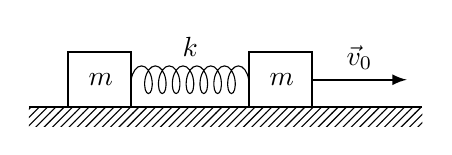
\begin{tikzpicture}

	\draw [draw=none, pattern=north east lines] (0,0) rectangle (5,-0.25);
	\draw [thick] (0,0) -- (5,0);
	\draw [thick] (0.5, 0) rectangle (1.3, 0.7) node [left=11pt, below=4pt] {$m$};	
	\draw [thick] (2.8, 0) rectangle (3.6, 0.7) node [left=11pt, below=4pt] {$m$};
	\draw [snake=coil, segment amplitude=5pt, segment length=5pt] (1.3,0.35) -- (2.8, 0.35) node [midway, above=5pt] {$k$};
	\draw [arrows={-latex}, thick] (3.6, 0.35) -- (4.8, 0.35) node [midway, above]  {$\vec{v}_0$};

\end{tikzpicture}
\end{document}